\section{Architektura}
Architektura platformy je tvořena z~několika částí, které jsou navzájem propojeny. Uživatel interaguje s~webovou aplikací, která komunikuje s~backendem. Backend je tvořen z~několika služeb, které komunikují s~datovými zdroji dopravců.
\begin{figure}[H]
    \centering
    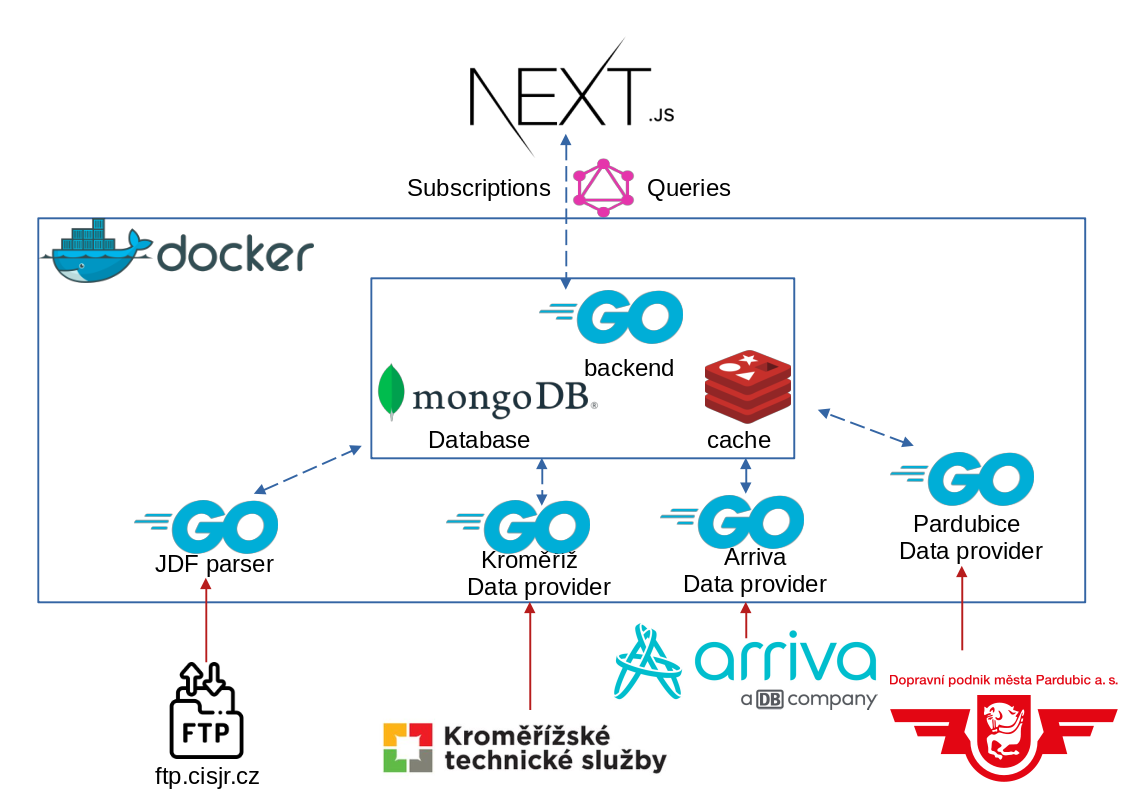
\includegraphics[width=0.75\textwidth]{images/architekturaV5.png}
    \caption{Architektura aplikace}
    \label{architektura}
\end{figure}
\newpage
Tento projekt je rozdělen do~dvou hlavních částí. První částí je frontend, vytvořený pomocí frameworku NextJS v programovacím jazyce TypeScript.
Druhou částí je backend, který je napsán v~programovacím jazyce GO.